% !TEX root = thesis.tex

\chapter{Data analysis}
\label{cha:data_analysis}
The datasets created allow to perform some measurement regarding the use of scholarly works in the English Wikipedia.
\todo{TODO\@: other statistics? Maybe some that use the pagecounts?}

\section{Wikipedia articles}
\subsection{Where do identifiers appear in a Wikipedia article?}

\subsection{How many sections Wikipedia articles have?}

\subsection{Which are the most common sections in Wikipedia articles?}

\section{Papers in Wikipedia}
This section analyzes the use of papers in wikipedia.

\subsection{Incoming citations distribution}
The distribution of scholarly citations has been studied many times by the scientific community.
The problem is to understand the law that describes the \emph{distribution of citations} of papers, namely the distribution of the number of papers $N(x)$ that have been cited $x$ times.
Redner~\cite{Redner1998} suggested that this distribution has a large-$x$ power law decay $N(x) \sim x^{-\alpha}$ \todo{explain some more of that article}.

Fig.~\ref{fig:incoming_citations_loglog} compares the distribution of citations of all the papers known to the MAG (circa 120 millions) and the ones whose \ac{DOI} appears in Wikipedia (circa 389 thousands).
The number of incoming citation for a paper is determined using the \ac{MAG} dataset.
Notice that the only identifier available in the \ac{MAG} is the \ac{DOI}, hence only the papers found in Wikipedia which have a \ac{DOI} are considered.
This accounts for the 28\% of the identifiers found.
Furthermore, from this set of papers we removed the ones that appears to be ``non-valid'' in the \ac{MAG} dataset, namely the ones that have more than one \ac{DOI}.
The amount of papers considered at the end is the 17\% of the identifiers found in Wikipedia.

From the graph we can only see that both the distribution follow some kind of power law.
It is more interesting to analyze the \ac{ccdf} of the two series.
In our case, the \ac{ccdf}, or \emph{tail distribution}, expresses the percentage of papers $\bar{F}(x)$ that have more than $x$ citations.

From Fig.~\ref{fig:incoming_citations_ccdf_1000}~and~\ref{fig:incoming_citations_ccdf_100} we can see that papers appearing in Wikipedia tend to have many more incoming citations with respect to a random paper taken from all the available ones.
For instance, the 74\% of papers in Wikipedia have at least 10 incoming citations, while only the 13\% of papers have at least 10 incoming citations.
A plausible explanation is that users tend to insert papers with a higher rank in term of incoming citations, rather than ones with less impact on the scientific community.
\todo{Regarding the ``All papers'' serie, should we limit only papers having DOIs?}
% see https://en.wikipedia.org/wiki/User:ProteinBoxBot.


\begin{figure}[h]
\centering
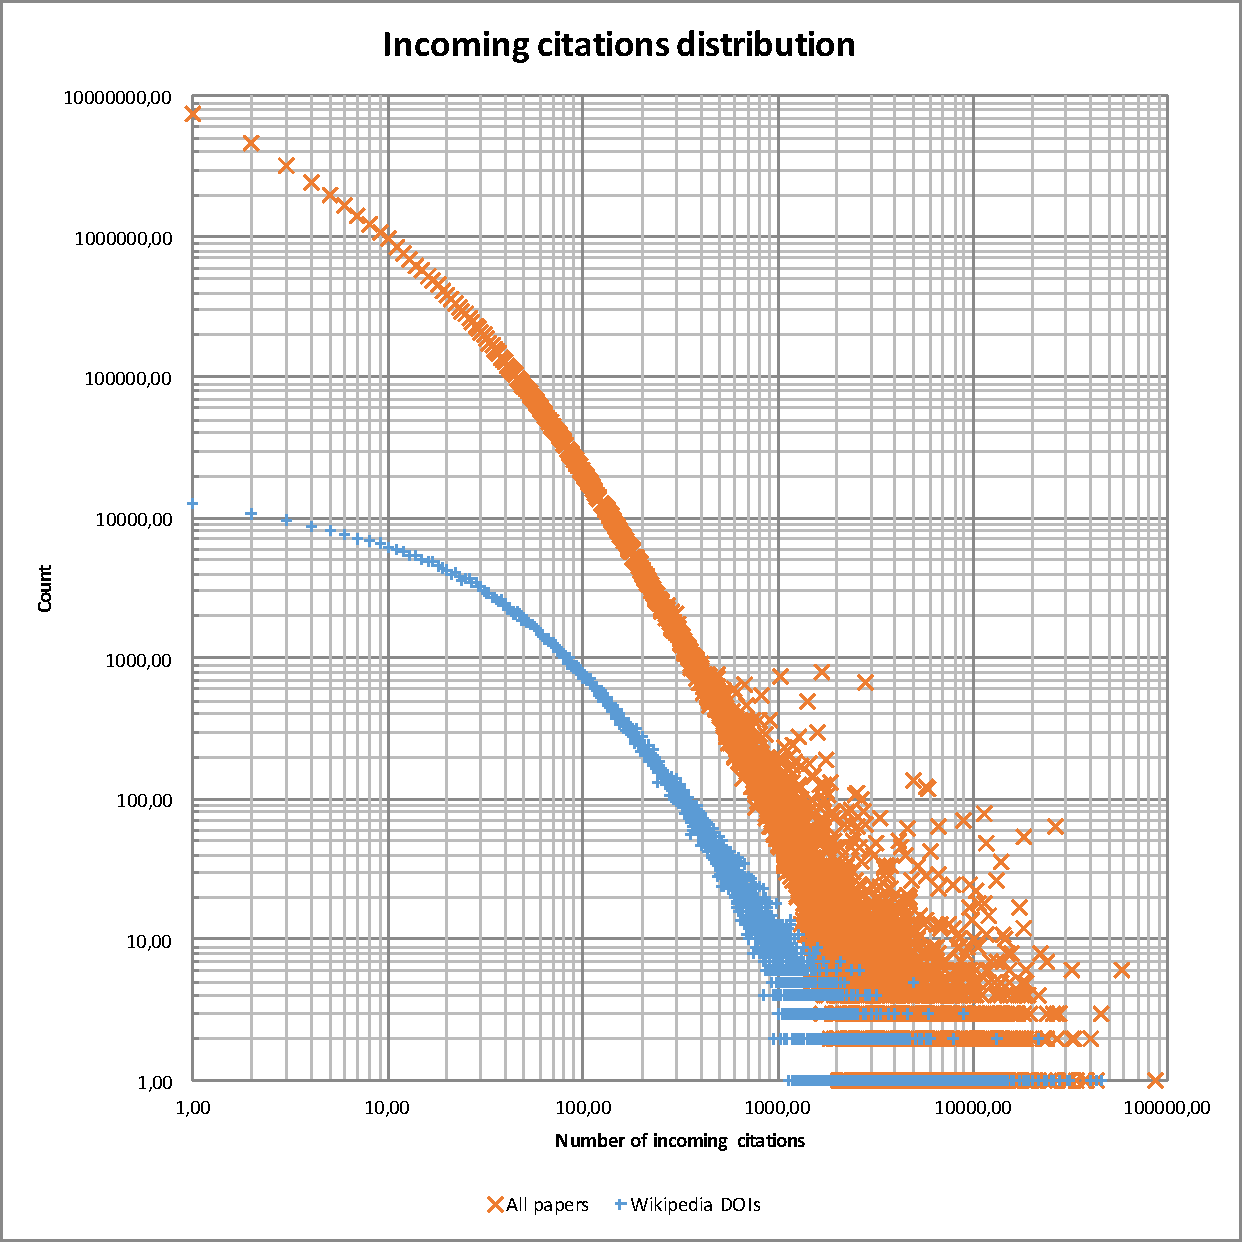
\includegraphics[keepaspectratio=true, width=\textwidth]{assets/incoming_cits_loglog}
\caption{Incoming citations distribution of papers appearing in the \emph{mag} datasets and the ones appearing only in English Wikipedia, on a log-log scale.}
\label{fig:incoming_citations_loglog}
\end{figure}

\begin{figure}[h]
\centering
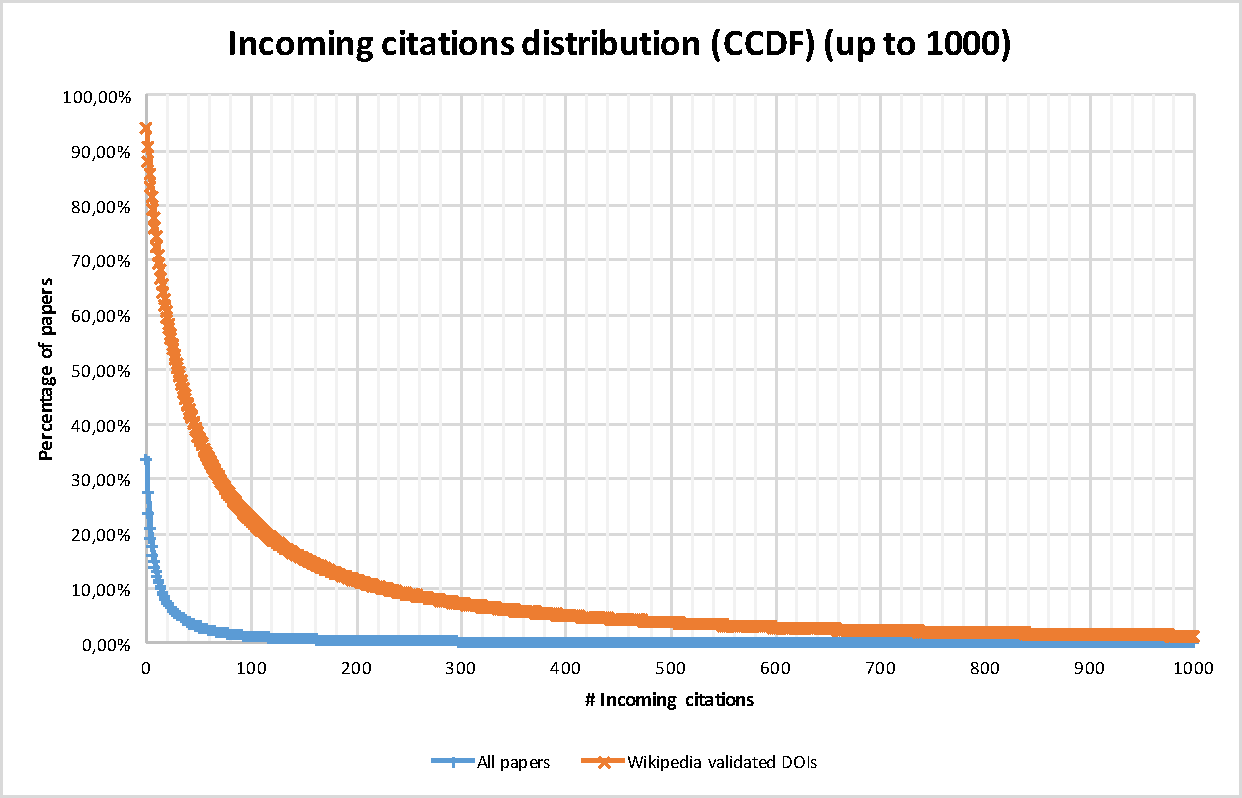
\includegraphics[keepaspectratio=true, width=\textwidth]{assets/incoming_cits_ccdf_1000}
\caption{Complementary cumulative distribution function of the first 100 incoming citations of papers appearing in the \emph{mag} datasets and the ones appearing only in English Wikipedia.}
\label{fig:incoming_citations_ccdf_1000}
\end{figure}

\begin{figure}[h]
\centering
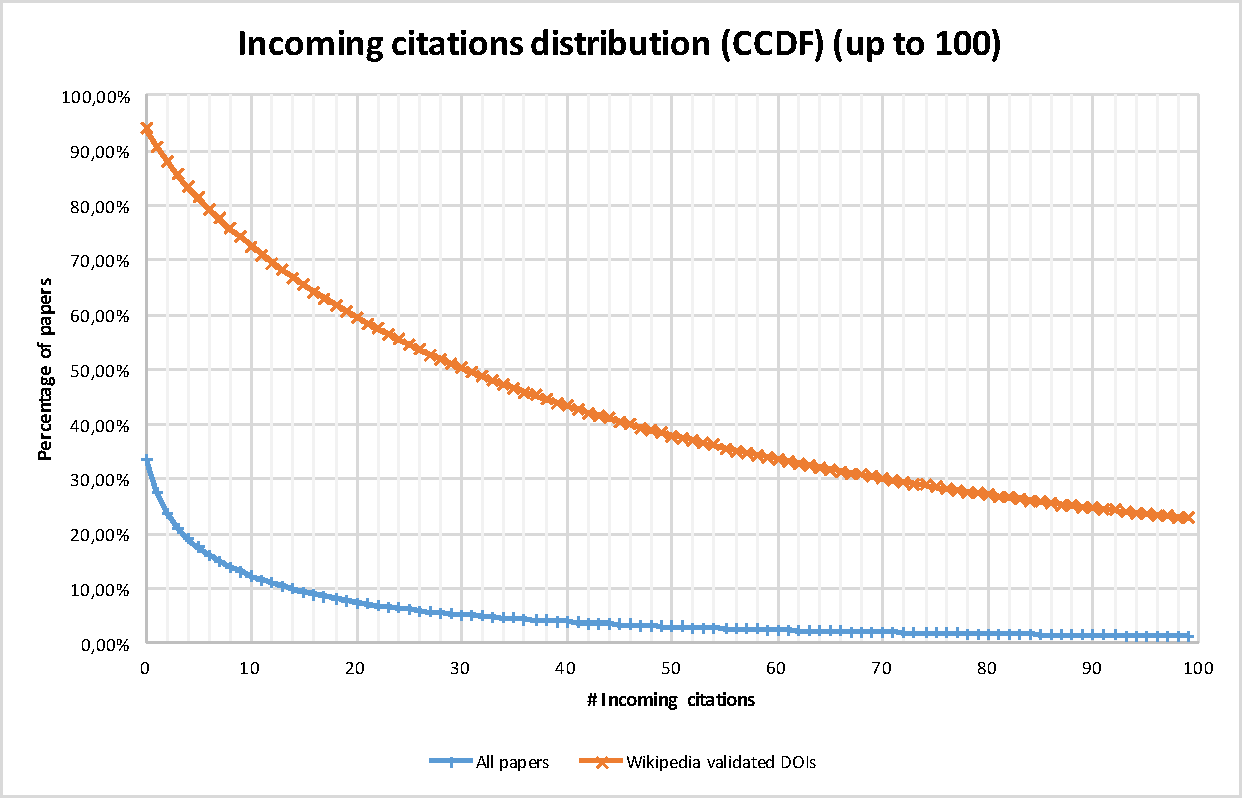
\includegraphics[keepaspectratio=true, width=\textwidth]{assets/incoming_cits_ccdf_100}
\caption{Complementary cumulative distribution function of the first 100 incoming citations of papers appearing in the \emph{mag} datasets and the ones appearing only in English Wikipedia.}
\label{fig:incoming_citations_ccdf_100}
\end{figure}

\subsection{Age of identifiers at first appearance}
Another interesting information to analyze is the age of the papers when they first appear in Wikipedia.
Fig.~\ref{fig:age_of_papers_at_first_appearance} shows the distribution of the age of papers when they are inserted on Wikipedia for the first time.
In theory there should not be negative values, because this would mean that an identifier appears in Wikipedia before the paper is published.
In practice this happens because the \ac{MAG} dataset is not 100\% accurate, and some publication dates may contain errors.
We have investigated this problem, and it seems to be caused by how Microsoft extracts the publication date of a paper.
It appears that if a paper is published online on a certain date, and it is also released after in a journal, Microsoft consider the date of the journal the publication date.
However, only the 3,12\% of the \acp{DOI} extracted have a negative age, so the effect of the error is arguably quite marginal.

It is interesting to see that many \acp{DOI} are inserted in Wikipedia few days after their publication (Fig.~\ref{fig:age_of_papers_at_first_appearance_zoom}).
We have analyzed some of these cases, and it appears that that some authors insert the identifier of their paper as soon as it has been published.

Finally, to give a scale to this numbers, Fig.~\ref{fig:age_of_papers_at_first_appearance_cdf} measure is the \ac{cdf} of the series, namely what is the percentage $F(x)$ of paper identifiers inserted in Wikipedia at most $x$ days after their publication.
\todo{conclude, somehow}

% Notes:
% Kamil Crater (doi 10.1126/science.1190990) has been added by the author as soon as possible. \url{https://en.wikipedia.org/w/index.php?title=Kamil_Crater&diff=next&oldid=375884625}

\begin{figure}[h]
\centering
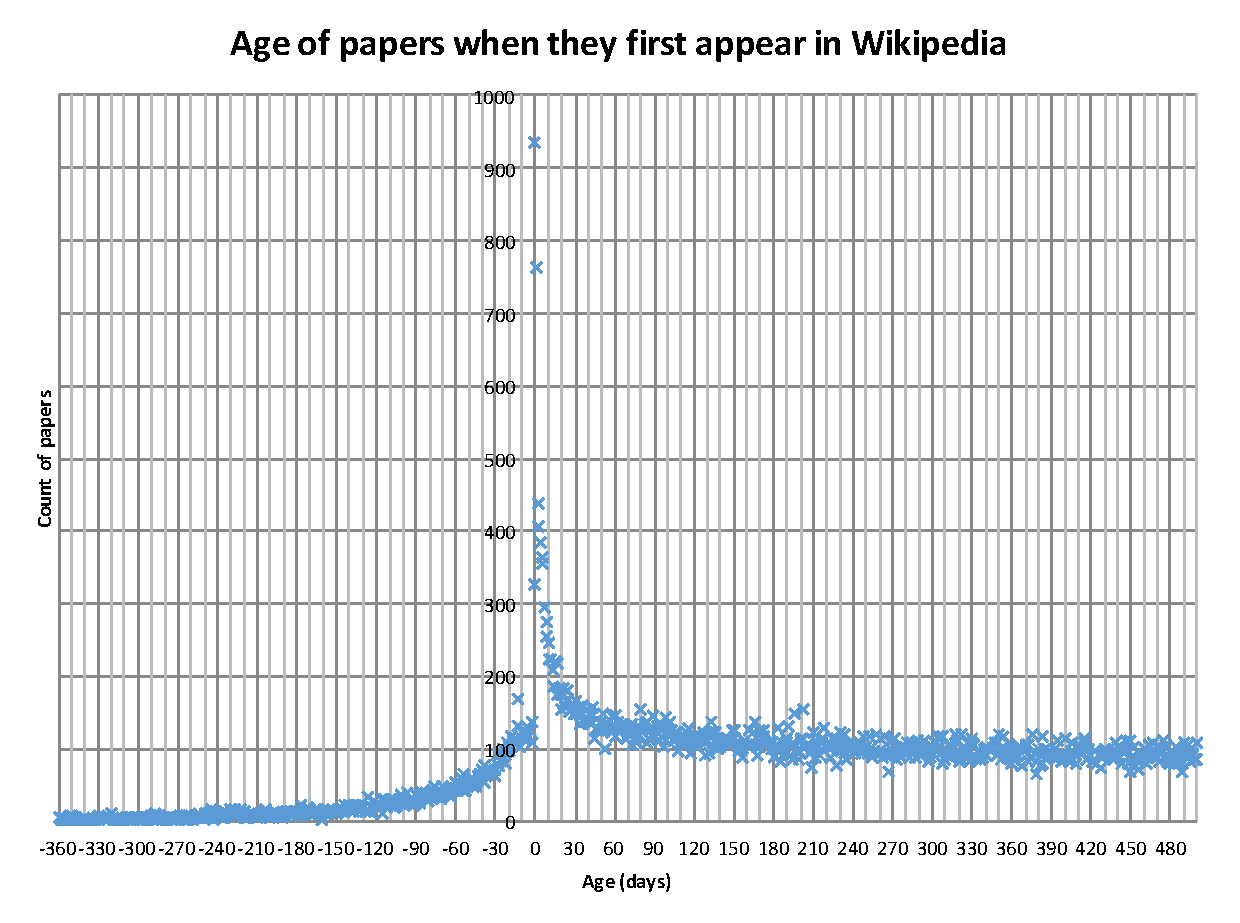
\includegraphics[keepaspectratio=true, width=\textwidth]{assets/age_of_papers_at_first_appearance}
\caption{Distribution of the age of papers when their DOI appear for the first time on Wikipedia.}
\label{fig:age_of_papers_at_first_appearance}
\end{figure}

\begin{figure}[h]
\centering
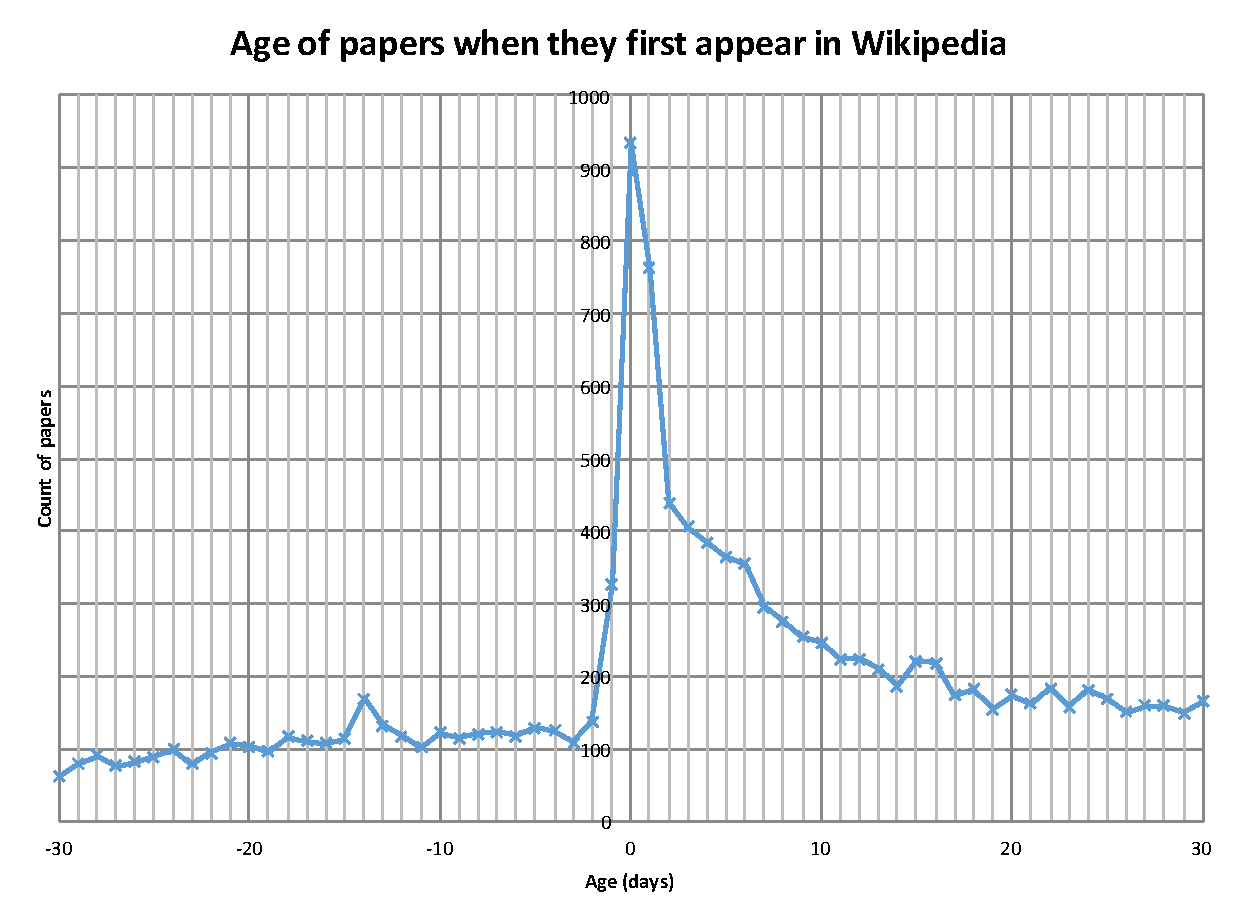
\includegraphics[keepaspectratio=true, width=\textwidth]{assets/age_of_papers_at_first_appearance_-30+30}
\caption{Distribution of the age of papers when their DOI appear for the first time on Wikipedia, showing only ages between $[-30, 30]$ days.}
\label{fig:age_of_papers_at_first_appearance_zoom}
\end{figure}

\begin{figure}[h]
\centering
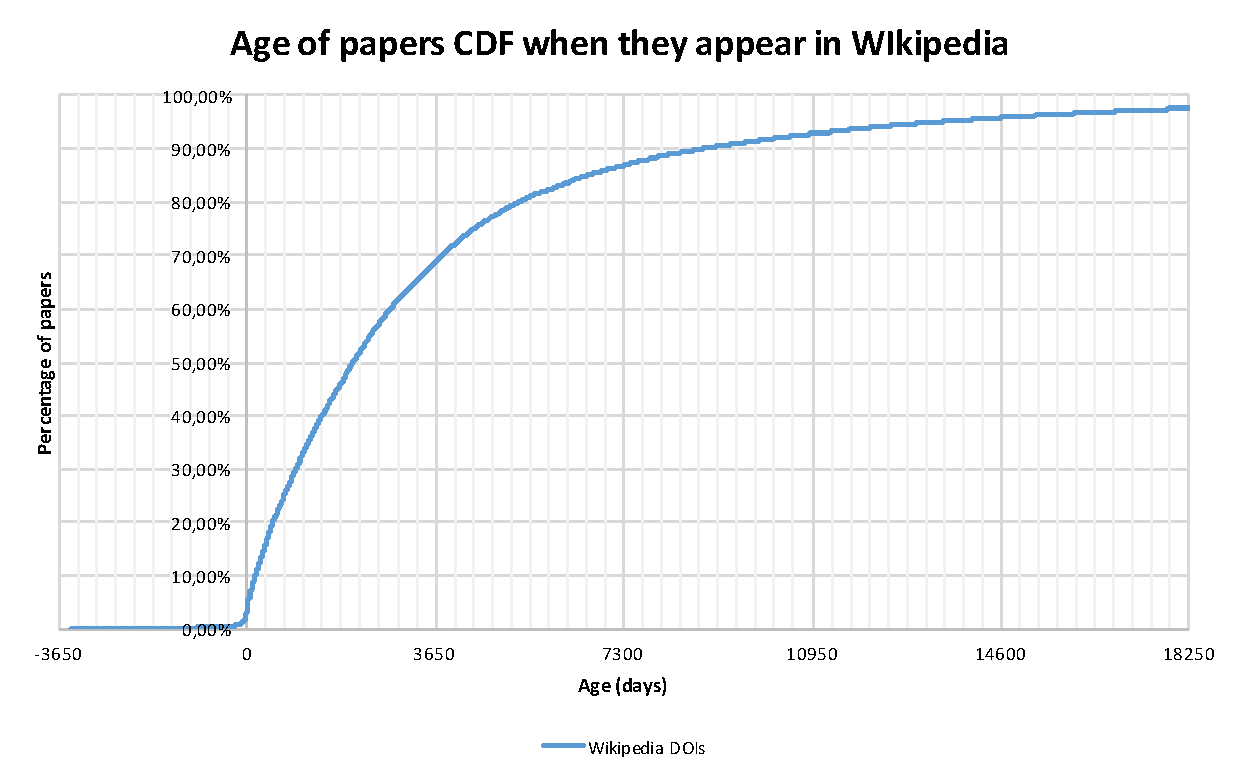
\includegraphics[keepaspectratio=true, width=\textwidth]{assets/age_of_papers_at_first_appearance_cdf}
\caption{todo}
\label{fig:age_of_papers_at_first_appearance_cdf}
\end{figure}

\subsection{Identifiers lifetime}
It is interesting also to analyze how long identifiers live inside a page.
In particular, the focus of this sections is on identifiers which have been inserted in a page and then removed for some reason, most probably because of irrelevance.
The rationale behind this choice is to analyze how long an irrelevant identifier stayed on a page before somebody removed it.

\begin{figure}[h]
\centering
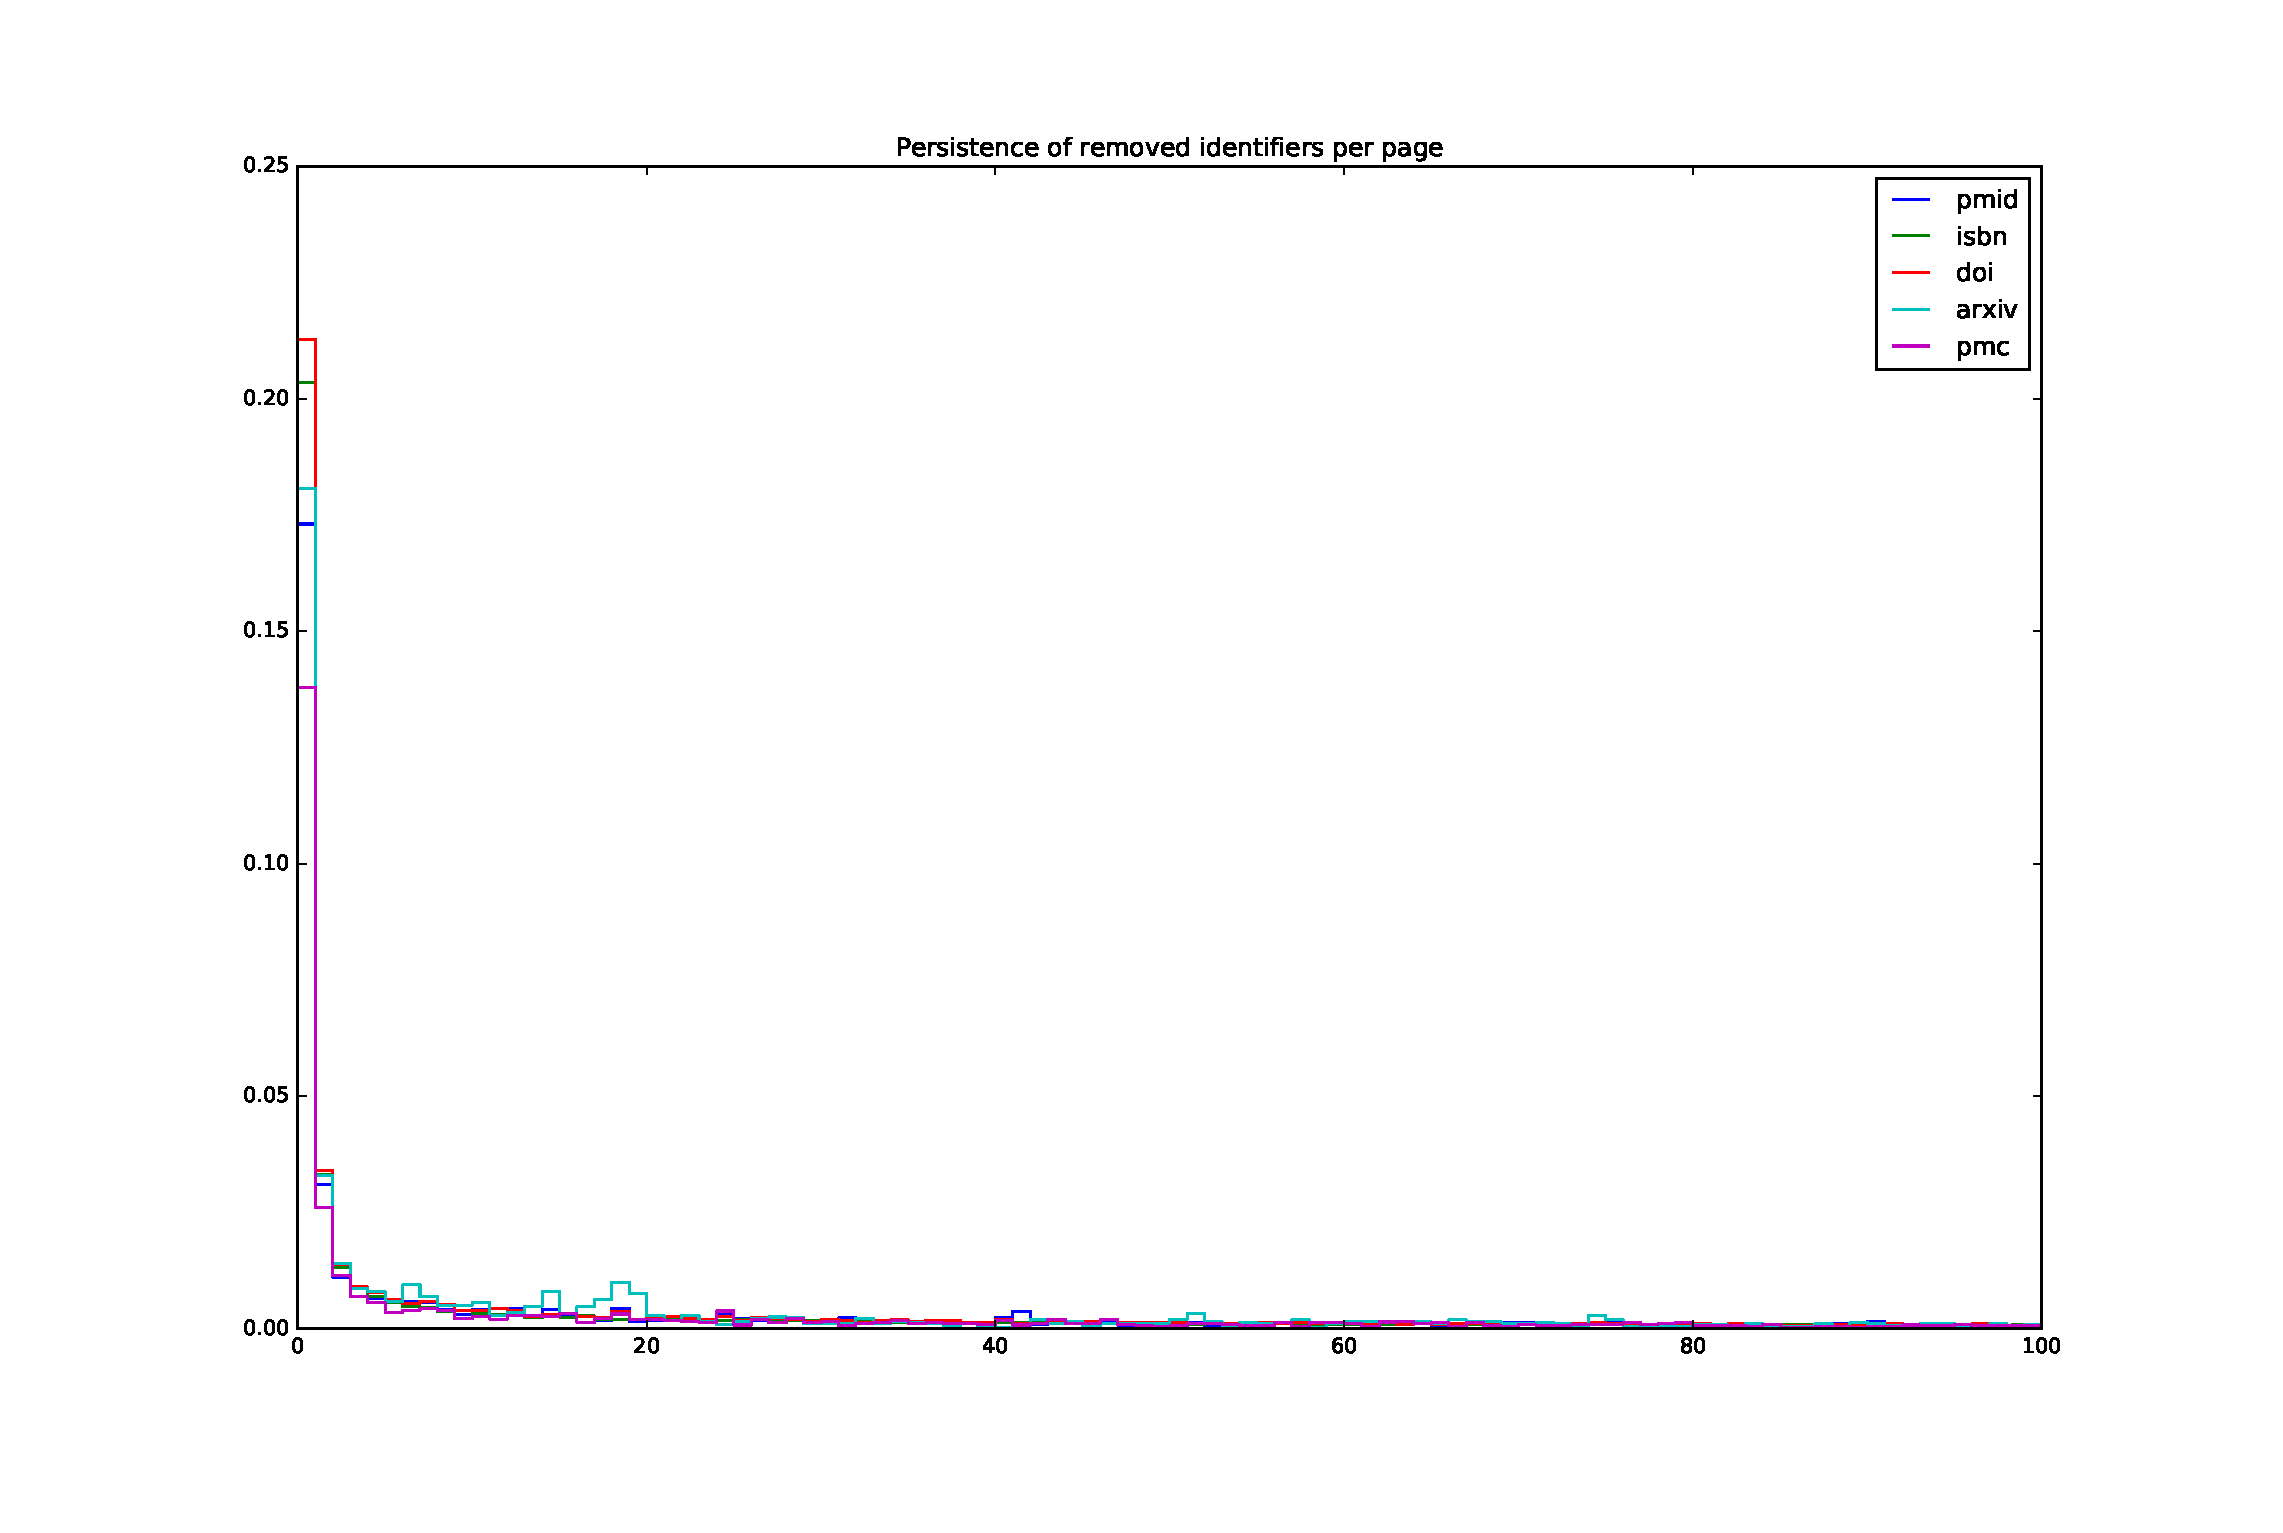
\includegraphics[keepaspectratio=true, width=\textwidth]{assets/persistence_removed_identifiers_pdf}
\caption{todo}
\label{fig:persistence_removed_identifiers_pdf}
\end{figure}

Fig.~\ref{fig:persistence_removed_identifiers_pdf} shows the \ac{pmf} of the lifetime of removed identifiers, aggregated by day.
Only the first 100 days are shown.
It is interesting to see that, for instance, more than the 20\% of the irrelevant \acp{DOI} are removed by the first day.

To get a more accurate idea of what is happening, Fig.~\ref{fig:persistence_removed_identifiers_cdf_days} shows the \ac{cdf} of these series.
The probability of removing an irrelevant identifier is fairly high in the beginning, but then it slowly decays.

\begin{figure}[h]
\centering
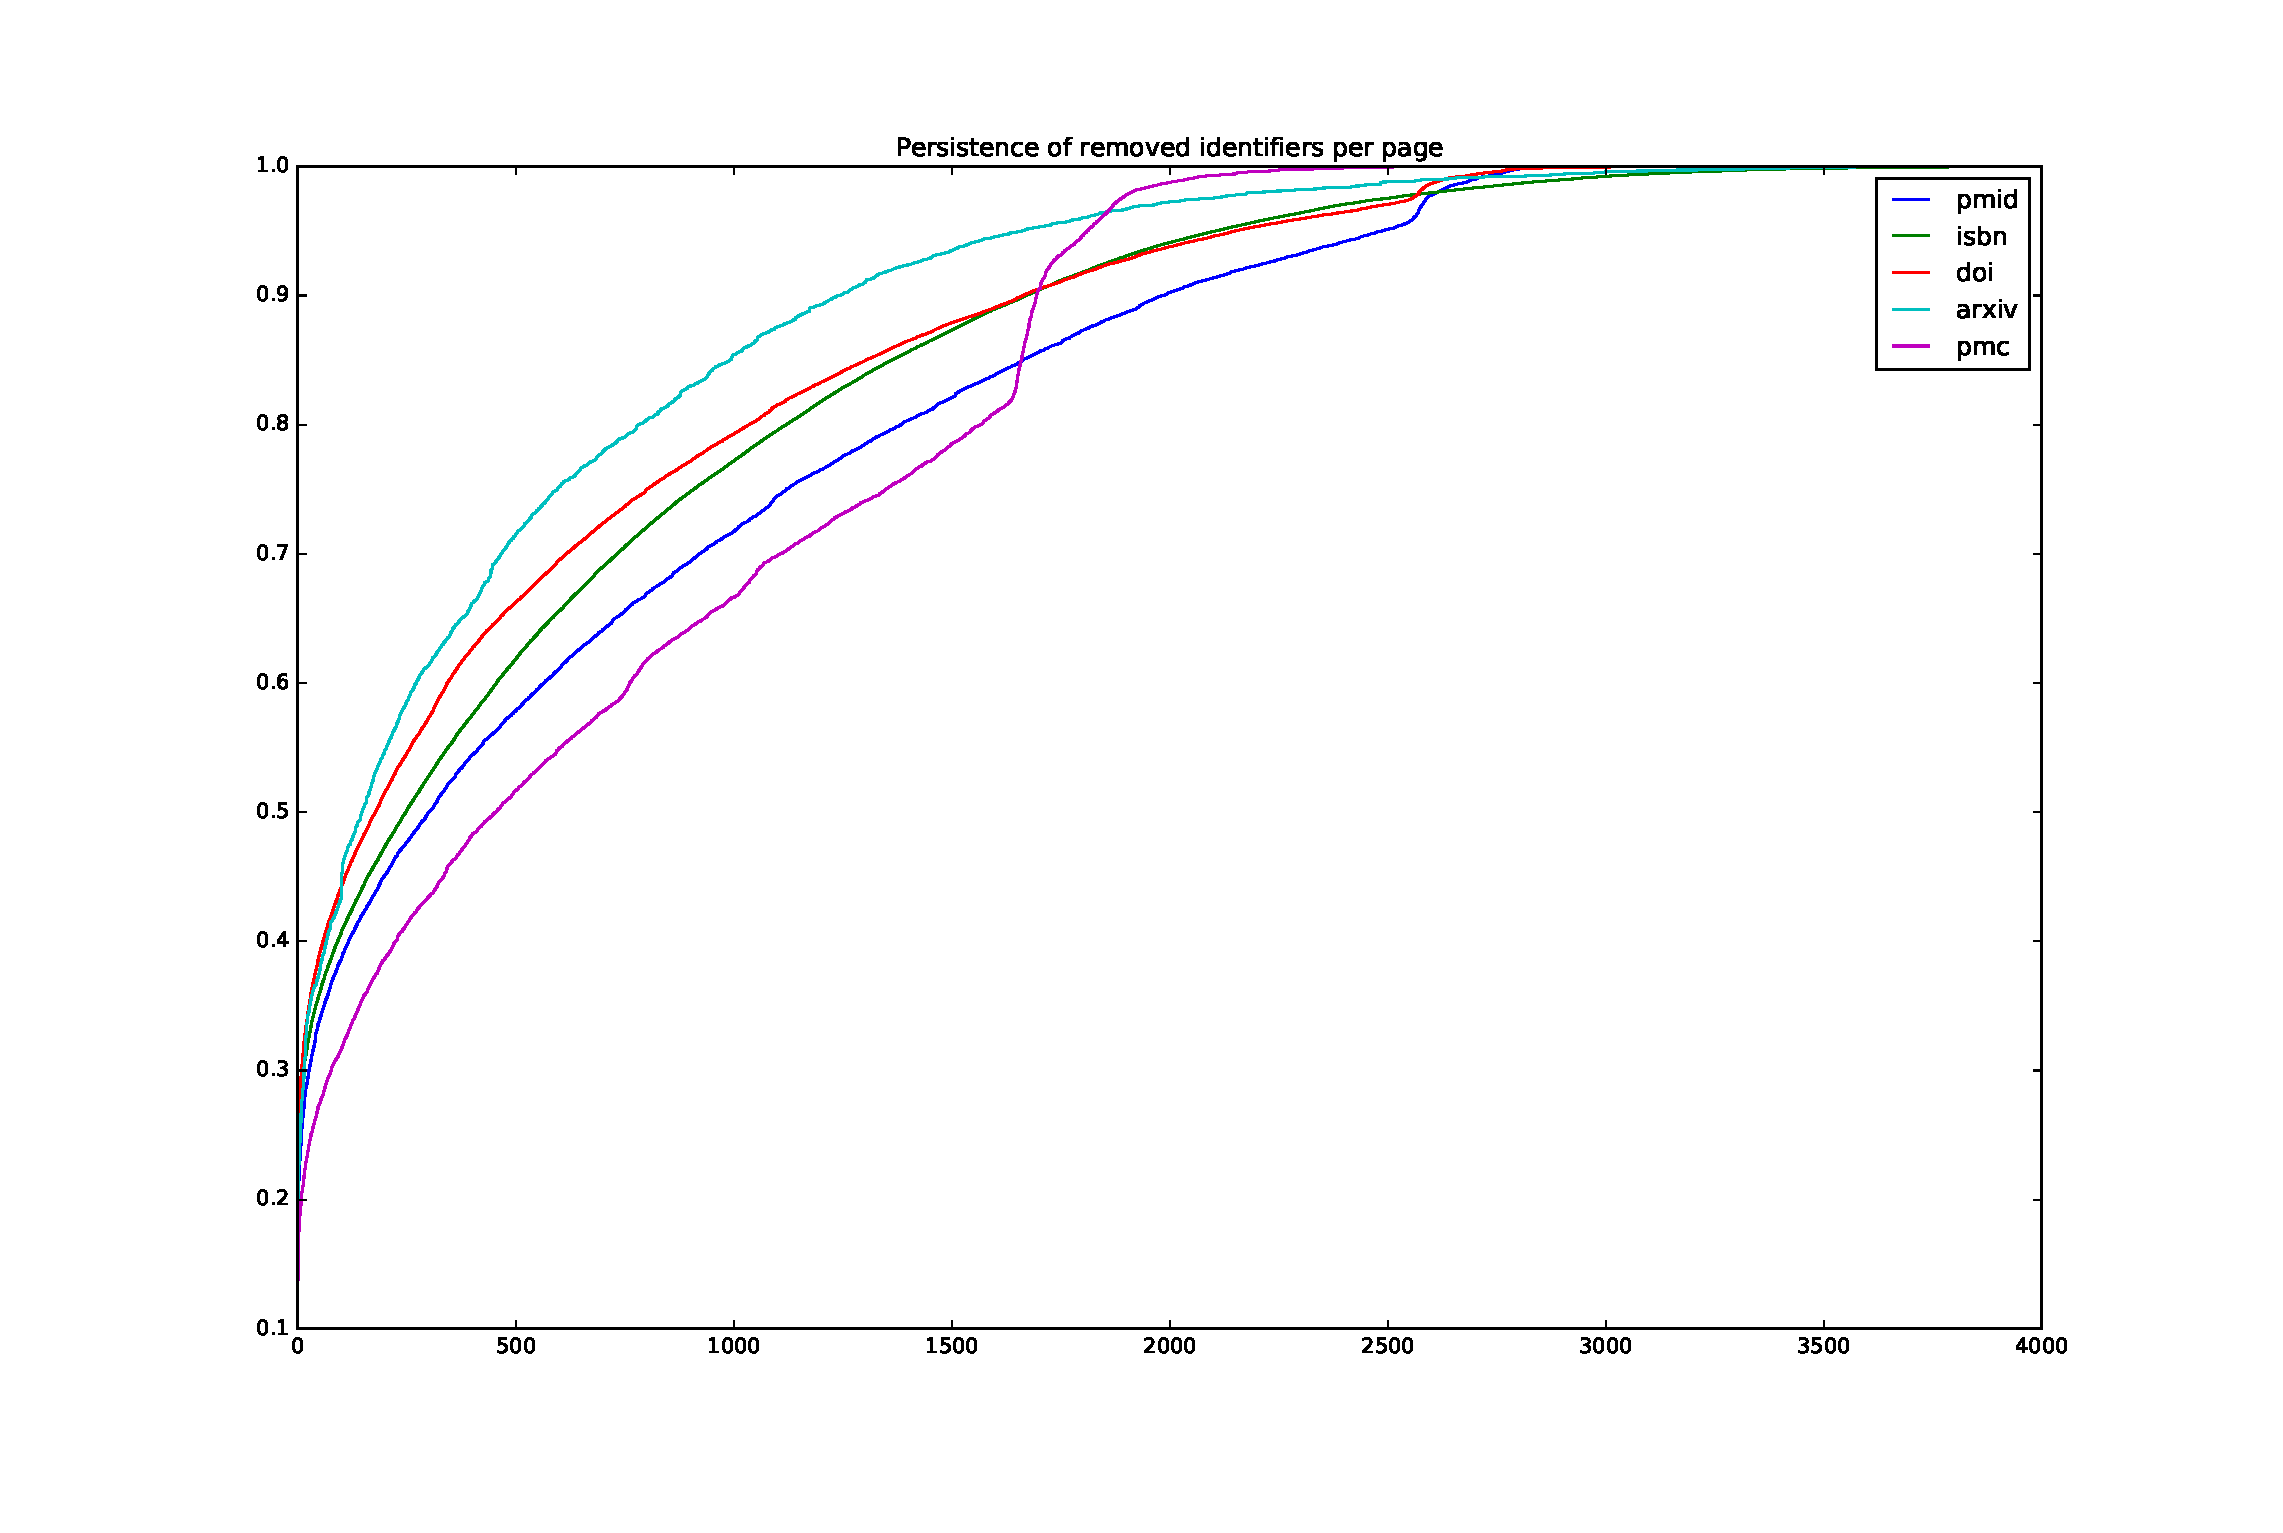
\includegraphics[keepaspectratio=true, width=\textwidth]{assets/persistence_removed_identifiers_cdf_days}
\caption{todo}
\label{fig:persistence_removed_identifiers_cdf_days}
\end{figure}

Fig.~\ref{fig:persistence_removed_identifiers_cdf_first_day} displays what happen in the first day.
We can see that about the 15\% of irrelevant identifiers are discovered and removed right from the first hour of their appearance in a page.

\begin{figure}[h]
\centering
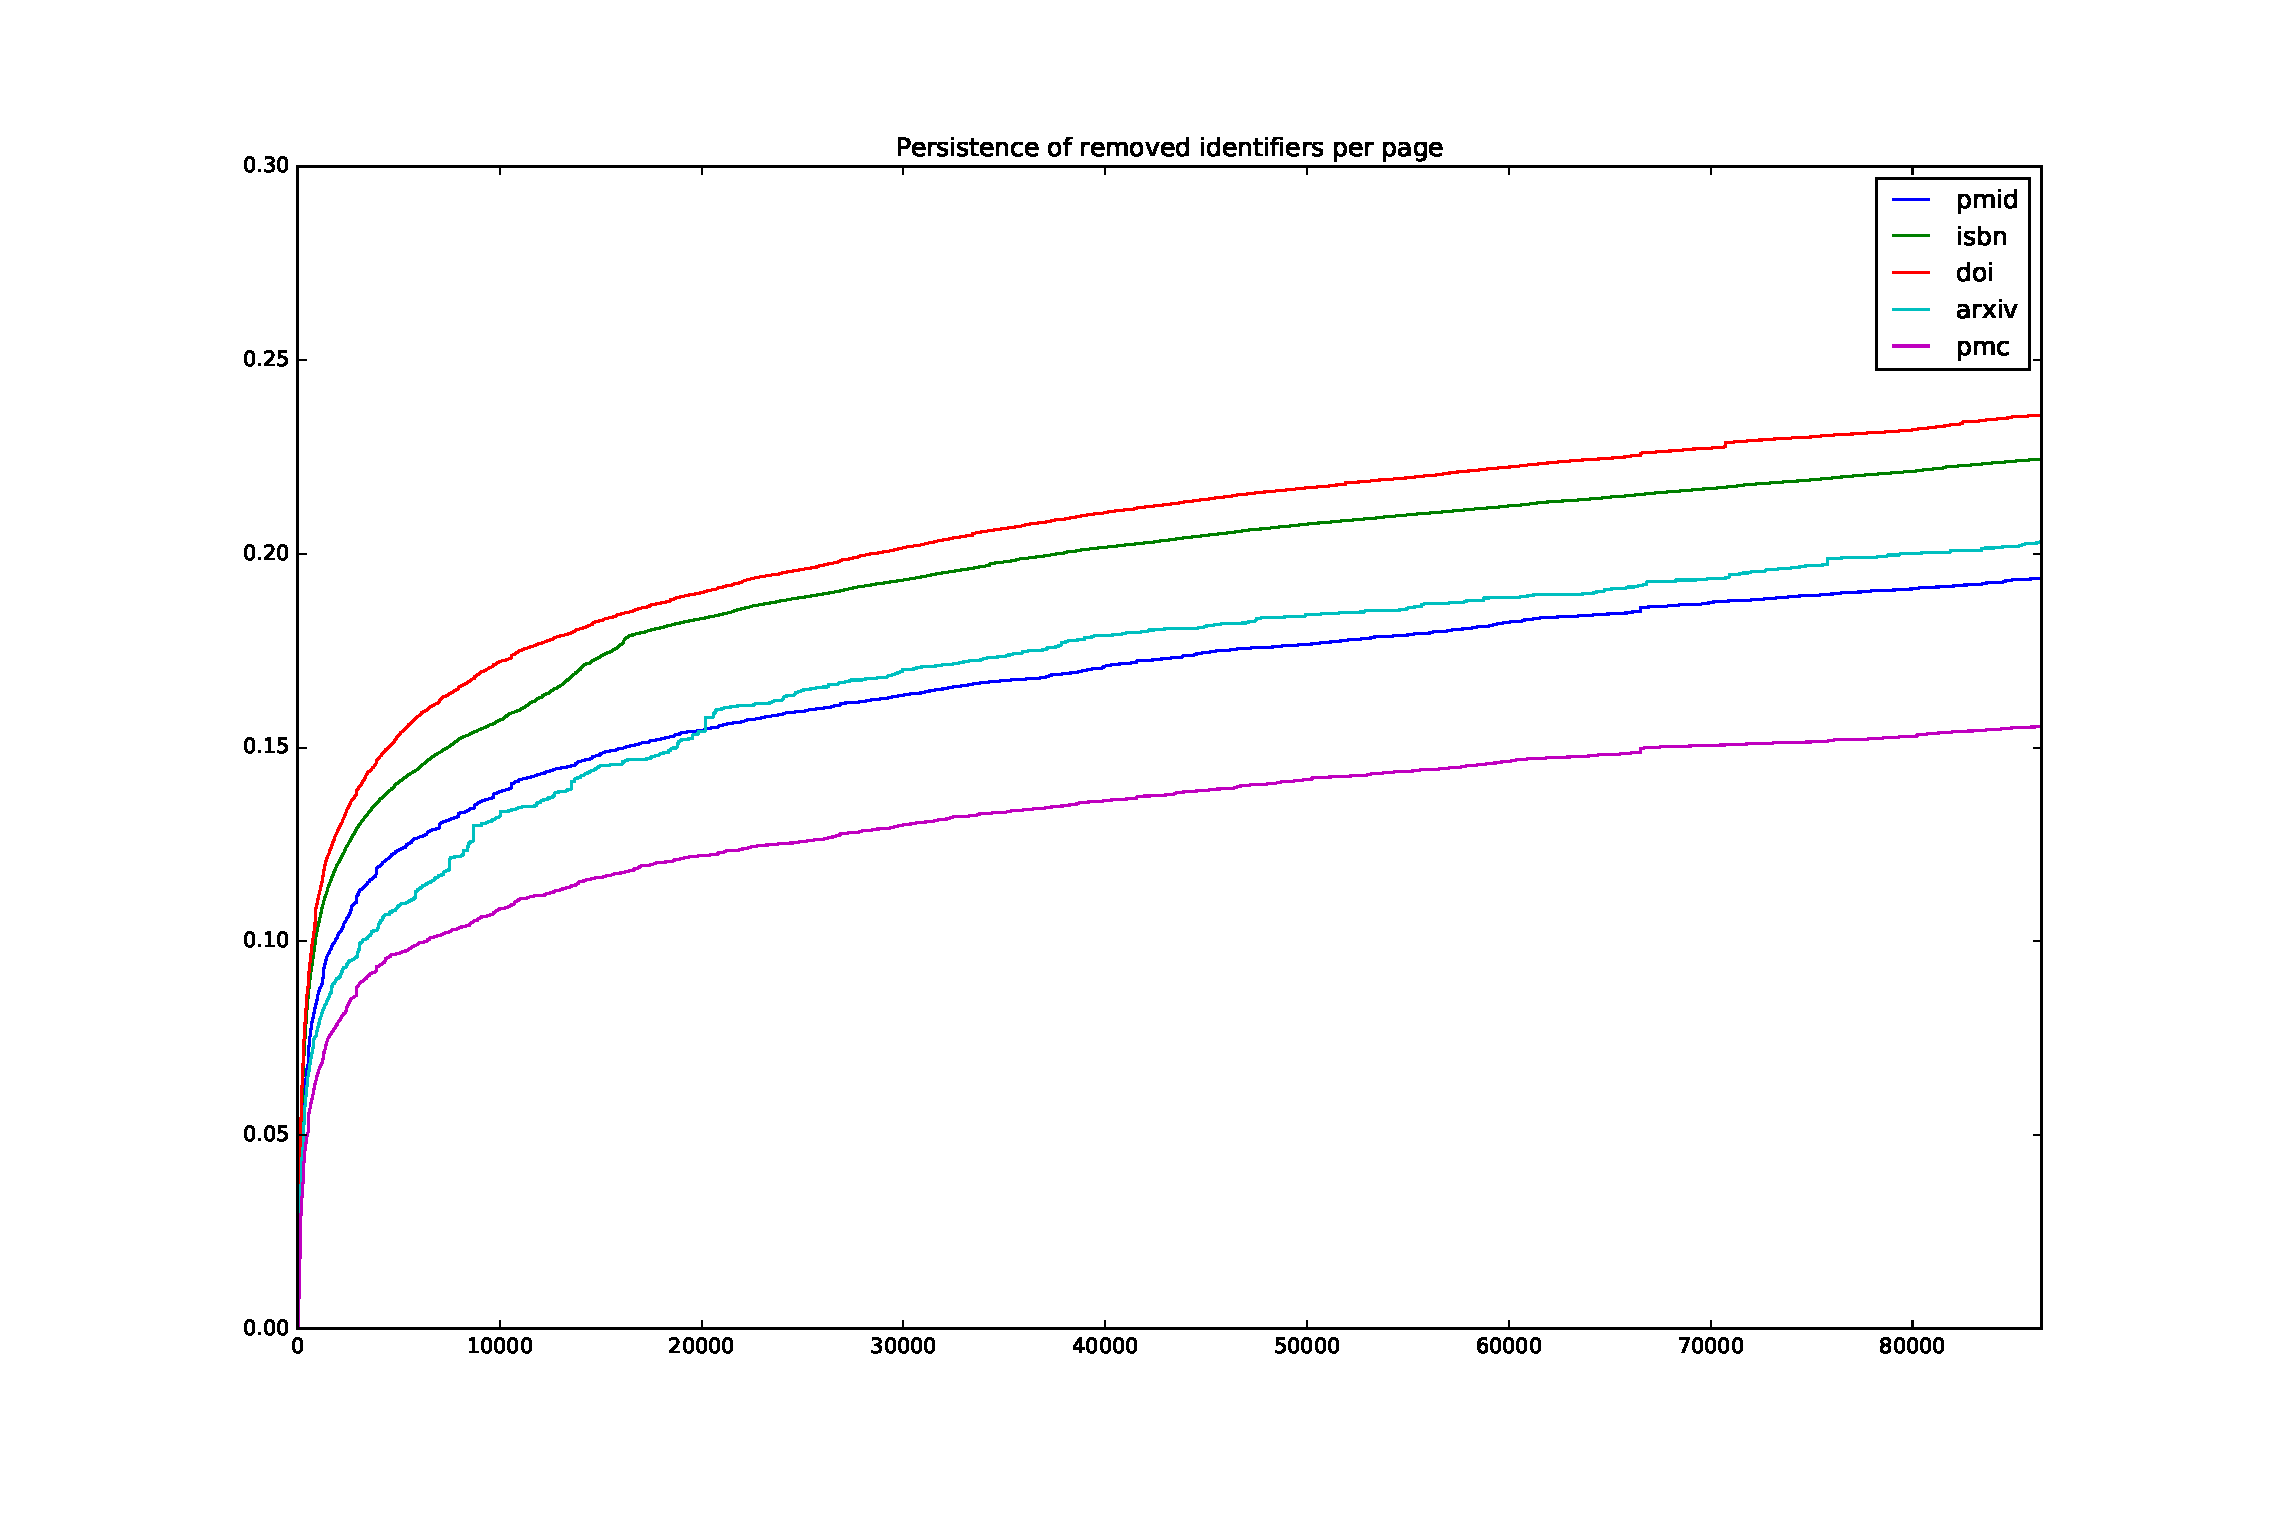
\includegraphics[keepaspectratio=true, width=\textwidth]{assets/persistence_removed_identifiers_cdf_first_day}
\caption{todo}
\label{fig:persistence_removed_identifiers_cdf_first_day}
\end{figure}

%A word of caution: we assume that if an identifier has been removed from a page and it is not present in the last revision at the time of the dump, then its appearance in the page is not relevant.

\subsection{Publication growth}
In 1961, Price~\cite{Price1961} studied the growth of scientific publications covering the period from about 1650 to 1950.
The data indicated a growth rate of about 5.6\% per year and a doubling time of 13 years.

The study of this matter has then been propose again by many, showing that the growth varies depending on the dataset used and analyzing different period of times.
For instance, Larsen et al.~\cite{Larsen2010} in the 2010 studied the growth using different datasets and limited to the time period between the 1907 and the 2007.
They showed that there are many other factors that determine the growth of publications that should be considered.

We have reproduced the result of Price, using the linear regression method, and we have obtained comparable results: the overall growth rate we have found is about 3,80\% and a doubling time of 18 years.
Fig.~\ref{fig:publication_date_regression} compares the actual growth with the one we have derived.

It is interesting to see also which is the distribution of the publication date of papers appearing in Wikipedia, and compare it with the distribution of the publication date of all the paper (Fig.~\ref{fig:publication_date_pdf}).
\todo{continue}


\begin{figure}[h]
\centering
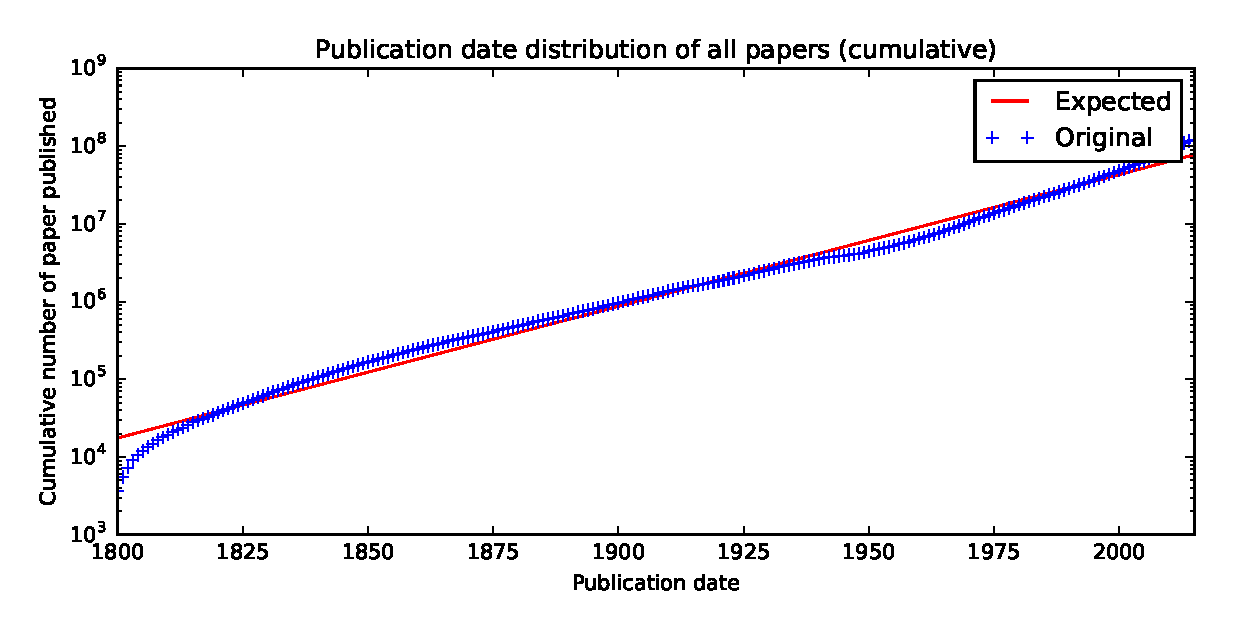
\includegraphics[keepaspectratio=true, width=\textwidth]{assets/publication_date_regression}
\caption{Publication date count for all the papers appearing in the \ac{MAG} dataset and its estimate curve obtained with linear regression}
\label{fig:publication_date_regression}
\end{figure}

\begin{figure}[h]
\centering
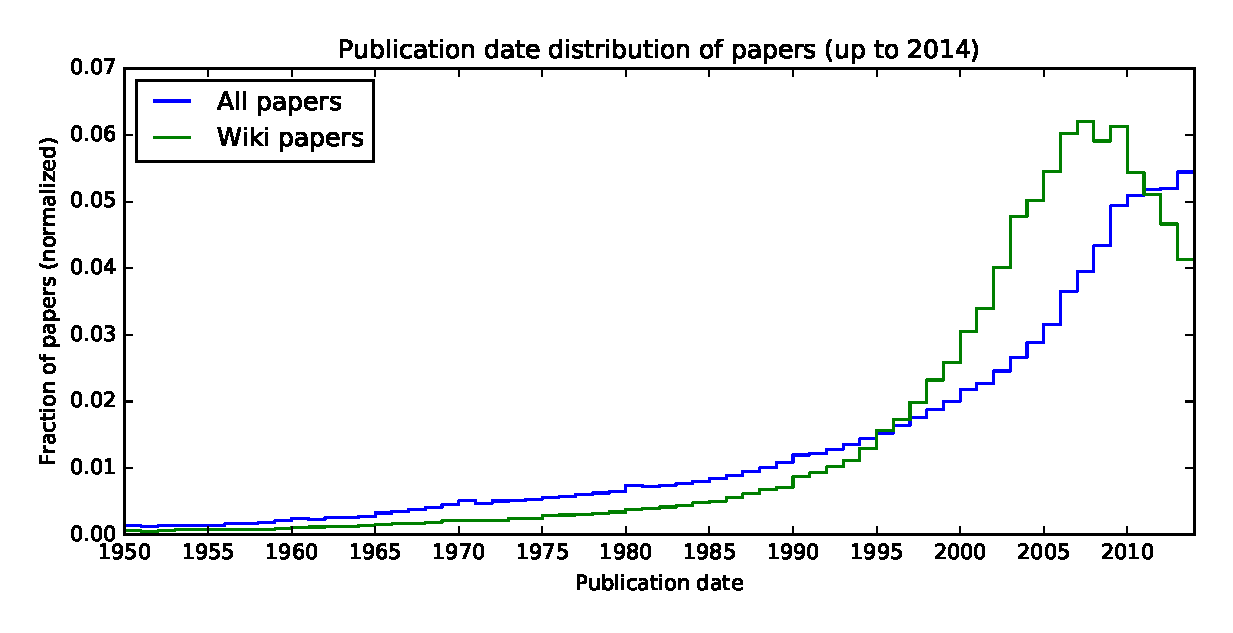
\includegraphics[keepaspectratio=true, width=\textwidth]{assets/publication_date_pdf}
\caption{Publication date distribution for all the known papers and for papers found in Wikipedia (only the ones having a DOI)}
\label{fig:publication_date_pdf}
\end{figure}

%\subsection{Top cited journals by views}
